%% Estuarine, Coastal and Shelf Science — elsarticle, author-year (Harvard)
%% Review mode: double-spaced, line numbers, single column.
%% Preamble mirrors reservoirs_s1_svm/manuscript/main.tex (Paper 1 and Paper 2).
\documentclass[review,12pt,authoryear]{elsarticle}

%% --- Encoding & fonts ---
\usepackage[T1]{fontenc}
\usepackage[utf8]{inputenc}
\usepackage{lmodern}

%% --- Math ---
\usepackage{amsmath,amssymb}

%% --- Graphics & tables ---
\usepackage{graphicx}
\graphicspath{{figures/}}
\usepackage{float}
\usepackage{booktabs}
\usepackage{tabularx}
\usepackage{longtable}
\usepackage{multirow}

%% --- Hyperlinks ---
\usepackage[hidelinks]{hyperref}
\usepackage{url}

%% --- Units ---
\usepackage{siunitx}
\sisetup{detect-all, group-separator={,}}

%% --- Misc ---
\usepackage{microtype}
\usepackage{lineno}       % line numbers (activated by 'review' class option)
\usepackage{setspace}
\usepackage[margin=2.5cm]{geometry}

%% --- Bibliography (natbib, Harvard author-year) ---
\biboptions{authoryear,round,semicolon}

% -----------------------------------------------------------------------
\begin{document}

\begin{frontmatter}

%% Chosen 2026-09-01, replacing the 2026-08-08 title, which named an
%% interaction between wave coupling and bed mobility. That interaction
%% survives only where the canopy is absent, so it can no longer sit in the
%% subject position.
%% "Relative" rather than "Interacting" is deliberate. The canopy is a clean
%% main effect, same sign in all four cells with every interval clear of zero,
%% and the word interacting would put the reader in the frame the paper
%% demotes. "Relative" promises the ranking the paper actually delivers.
%% "Vegetated" is dropped because "seagrass canopy" already carries it.
\title{Relative effects of seagrass canopy, wave coupling and bed mobility on
       Lagrangian transport in a shallow lagoon}

%% Nasello and Maltese added on De Marchis's review of 2026-10-13. Three points
%% still need the authors' own confirmation before submission, because Elsevier
%% requires written agreement from every author for any change before
%% acceptance and permits none after it:
%%   (i)   the order below, De Marchis, Ciraolo, Nasello, Maltese after the
%%         corresponding author, was set by the corresponding author on
%%         2026-10-15 and still needs the agreement of the others;
%%   (ii)  Nasello and Maltese are assumed to be at Dipartimento di Ingegneria;
%%   (iii) the CRediT roles follow the reservoirs_s1_svm pattern for
%%         supervising co-authors, with Methodology for Maltese on the strength
%%         of the classification approach Section 3.4 builds on.
\author[unipa]{Cicero Martins Jr.\corref{cor1}}
\ead{cicero.martinsjr@unipa.it}

\author[unipa]{Mauro De Marchis}
\author[unipa]{Giuseppe Ciraolo}
\author[unipa]{Carmelo Nasello}
\author[unipa]{Antonino Maltese}

\cortext[cor1]{Corresponding author}
\affiliation[unipa]{organization={Dipartimento di Ingegneria,
                    Università degli Studi di Palermo},
                    city={Palermo},
                    country={Italy}}

% -----------------------------------------------------------------------
\begin{abstract}
%% About 245 words. ECSS limit is 250.
Coastal lagoon models are routinely validated against water level, although
habitat connectivity and dispersal depend on transport. This study asks which
modelled processes control transport in a shallow vegetated lagoon and whether
water level can identify them. A three-dimensional Delft3D Flexible Mesh model
of the Stagnone di Marsala, a micro-tidal Sicilian lagoon of sub-metre mean
depth colonised by \emph{Posidonia oceanica}, was coupled to SWAN over nine days
of July 2025. Eight configurations form a complete factorial in wave coupling,
bed mobility and seagrass canopy, with the canopy parameterised from published
measurements and distributed by satellite classification, and each was scored
against three tide gauges and 35 GPS surface drifters withheld from every model
decision. On the fixed bed, Liu--Weisberg skill ranges from 0.597 to 0.739 and
divides on the canopy, which raises it by 0.120 and 0.114 with both bootstrap
intervals clear of zero, against $-0.022$ and $-0.028$ for wave coupling. Water
level separates the canopy treatments only at the gauge inside the vegetated
basin, by 26 and 27~mm in anomaly RMSE against at most 4~mm near the inlets.
With waves, the uncalibrated mobile bed brings a configuration without canopy to
the skill of the vegetated ones through a bathymetry reshaped by implausible
erosion, a compensation that the interior gauge exposes and the drifters do not.
The canopy is therefore the first-order control on transport here, and leaving
it out lets errors elsewhere pass as process effects. These results rest on one
nine-day window and a stratified initial state. Transport prediction in
vegetated lagoons requires canopy drag resolved rather than absorbed into bed
roughness, and published measurements with satellite mapping suffice to specify
it without tuning.
\end{abstract}

%% ECSS allows 1-7 keywords. Avoid multi-word keywords joined by 'and'/'of'.
\begin{keyword}
Coastal lagoon \sep
Delft3D Flexible Mesh \sep
Canopy drag \sep
\emph{Posidonia oceanica} \sep
Lagrangian drifters \sep
Three-dimensional circulation
\end{keyword}

\end{frontmatter}

\linenumbers   % activate line numbering for review

% -----------------------------------------------------------------------
\section{Introduction}
\label{sec:introduction}

Coastal lagoons are among the most productive coastal environments on Earth,
concentrating fisheries and biodiversity along roughly 13\% of the global
shoreline \citep{Carrasco2016, Kjerfve1994}. The shallow, semi-enclosed
geometry that sustains this productivity also makes them acutely sensitive to
the atmospheric and tidal forcing that drives water exchange and renewal. In
the Mediterranean, where tidal amplitudes rarely exceed 0.3~m, the balance
among tide, wind stress and seiches varies from one lagoon to another, but wind
consistently emerges as a significant driver of horizontal exchange, and
through it of the residence times and salinity gradients that condition benthic
habitat \citep{Niedda2007, Umgiesser2014}. In many of these lagoons that
habitat is seagrass, principally \emph{Posidonia oceanica} (L.) Delile and
\emph{Cymodocea nodosa} (Ucria) Ascherson, and the relation runs in both
directions, since the canopies that depend on the circulation also act on it,
attenuating incident wave energy \citep{Infantes2012} and extracting momentum
from the mean flow through a drag that modifies near-bed turbulence and the
vertical velocity structure \citep{Nepf2012}. These meadows are declining,
global seagrass extent having fallen in all seven bioregions, by 19.1\% of the
surveyed area since 1880 \citep{Waycott2009, Dunic2021}, with the fastest
recent losses where meadows are exposed to coastal development and degraded
water quality \citep{Turschwell2021}. How circulation sets residence times,
dispersal and habitat connectivity in vegetated lagoons is therefore a question
for management as much as for science, and it concerns transport pathways, a
quantity that water level, the usual validation target of lagoon models, does
not measure directly.

The \emph{Stagnone di Marsala}, on the north-western coast of Sicily, is a
lagoon of this kind. Its mean depth is about 0.95~m, and its floor is largely
covered by meadows of \emph{P.\ oceanica} and \emph{C.\ nodosa}
(Section~\ref{sec:study_area}). Satellite monitoring over 2003--2024 has
documented a 75\% reduction in the extent of the \emph{P.\ oceanica} atoll and
cordon formations \citep{Maltese2025}, so the vegetated state a model of this
system must represent is itself changing.

Numerical studies of the Stagnone have each been built around the question they
addressed. \citet{LaLoggia2004} and \citet{DiMarca2009} used depth-averaged
models to characterise tidal flushing, residence times and turbidity, for which
the basin-scale water budget is the relevant quantity, and
\citet{Ciraolo2009a} showed through particle tracking how strongly simulated
trajectories depend on the velocity field they are advected through.
\citet{DeMarchis2012} resolved the vertical and showed that wind drives a
recirculation with a near-bed return flow even at sub-metre depths, with the
meadow represented through Nikuradse roughness heights assigned by seagrass
class and the model validated against velocity and water level at several
stations. \citet{Ingrassia2024} calibrated a depth-averaged model against water
level for a range of vegetation scenarios, a setting in which a uniform
equivalent roughness is the appropriate representation of the canopy. Building
on these studies, three aspects of the problem remain open for this basin. The
first is the representation of the canopy as a drag resolved over the vertical
extent of the plants, a formulation that acts on the shape of the velocity
profile as well as on its magnitude \citep{Nepf2012} and that is now available
in three-dimensional solvers. The second is the effect of waves, which in
comparably shallow Mediterranean lagoons alter bed stress and mobilise sediment
\citep{Carniello2011, Morote2025}, together with that of a bed evolving under
their combined action with the currents. The third is the assessment of
transport itself, the models having been evaluated mainly on water level and on
currents at fixed stations. Whether a model that reproduces water level also
reproduces transport, and which of the processes it carries are responsible
when it does, therefore remains to be established for this basin, and the
question extends to shallow vegetated lagoons in general, where Lagrangian
observations are known to constrain a model differently from water level
\citep{Liu2011, Revelard2021}.

The study takes up these three aspects by separating, in a three-dimensional model of
the Stagnone, the contributions of the canopy, of wave coupling and of bed
mobility, and by scoring every combination of the three against both water
level and observed drifter trajectories (Section~\ref{sec:data_methods}). It
pursues three objectives. The first is to rank the three processes by their
effect on Lagrangian transport skill. The second is to establish whether water
level, the quantity against which shallow lagoon models are conventionally
validated, can identify that ranking. The third is to measure how far the
apparent effect of each process depends on how the other two are represented.
The second and third are not specific to this basin, concerning what a class of
validation data can certify and how a factorial behaves when a dominant factor
is left out of it.

\section{Study Area}
\label{sec:study_area}

The \emph{Stagnone di Marsala} is located on the north-western coast of
Sicily, sheltered from the western Sicilian channel by Isola Grande, an
elongated barrier island running parallel to the mainland coast
(Figure~\ref{fig:study_area}). The enclosed basin extends approximately 11~km
in the north--south direction and 2.5~km east--west, enclosing a total surface
area of roughly 2200~ha \citep{DeMarchis2012}. Two geomorphologically distinct
sub-basins are separated by a \emph{Posidonia oceanica} barrier reef
\citep{LaLoggia2004}: the northern sub-basin, with a mean depth of
approximately 1~m and extensive intertidal flats, and the deeper southern
sub-basin, with a mean depth of approximately 2~m and a maximum of about 3~m
near the main inlet. Three islands punctuate the interior, the Phoenician
archaeological site of Mothia in the south-central basin and the smaller
islands of Santa Maria and Scuola in the central reaches
\citep{CiraoloDeMarchis2009}. Salt pans (\emph{saline}) occupy both margins of
the lagoon, with extensive historic saltworks on the western barrier island
(Isola Grande) and additional pans along the eastern mainland shore in the
area facing Mothia \citep{Basso2008}. They constitute a distinctive shallow
intertidal habitat within the lagoon system.

Hydrodynamic exchange with the open sea occurs through two morphologically
distinct inlets. The northern inlet (approximately 400~m wide, 0.30--0.40~m
deep) is a highly restricted passage whose tidal prism is severely limited by
its shallow sill. A historically dredged channel (20~m wide, 1~m deep)
partially compensates this restriction \citep{CiraoloDeMarchis2009}. The wide
southern inlet (approximately 2900~m wide, 1.0--1.5~m deep) provides the
primary pathway for mass transport and water mixing between the lagoon and the
open sea \citep{CiraoloDeMarchis2009}. The tidal regime is microtidal, with
free-surface amplitudes of approximately 0.30~m dominated by semi-diurnal
harmonics \citep{LaLoggia2004}. In the absence of riverine input, weak tidal
exchange combined with high summer evaporation drives a pronounced salinity
gradient. Annual lagoon-wide salinity spans 33--46~psu \citep{Basso2008}, with
peak summer values approaching 48~psu in the more confined northern sub-basin,
contrasting with near-marine conditions near the southern inlet
\citep{Mancuso2023}. Wind forcing dominates east--west circulation within the
basin, while tidal exchange controls the north--south component
\citep{CiraoloDeMarchis2009, DeMarchis2012}.

The seagrass mosaic covers the majority of the lagoon floor.
\emph{Posidonia oceanica} occupies the central and southern portions of the
basin, forming both continuous meadows and characteristic atoll patterns
(10--20~m in diameter) that grade into reef formations oriented along the
north--south axis. \emph{Cymodocea nodosa} prevails in the shallower northern
reaches, with \emph{Caulerpa prolifera} replacing \emph{P.\ oceanica} locally
where hydrodynamic and sediment conditions deteriorate
\citep{LaLoggia2004, CiraoloDeMarchis2009}. In Mediterranean meadows of this
type, \emph{P.\ oceanica} areal density reaches
1000--1200 plants~\si{\per\metre\squared} \citep{Ciraolo2009a}. The spatial
distribution of submerged vegetation was first mapped from airborne
hyperspectral imagery by \citet{CiraoloMaltese2006}. The roughness
parametrisation in this study rests on an independent classification of
PlanetScope imagery for the 2023 epoch, described in
Section~\ref{sec:methods_roughness}. The lagoon is designated both as a
\emph{Riserva Naturale Orientata} and as a Natura 2000 site, reflecting the
conservation importance of these meadows. The extent of the atoll and cordon
formations nevertheless fell by approximately 75\% between 2003 and 2024
\citep{Maltese2025}.

The observational dataset used in this study was collected during July 2025
(Figure~\ref{fig:study_area}). Water level was recorded at three stations,
BocaNord (BN) at the northern inlet, BocaSud (BS) near the southern inlet, and
AltaVilaEst (AE) on the eastern flank of the central basin. Wind speed and
direction and atmospheric pressure were measured at two stations, AE (which
also carries a water-level gauge and a water temperature sensor) and Mulino, a
dedicated meteorological station located near the salt pans in the
central-northern area. Water levels at BN, BS, and AE serve as the primary
validation targets for the hydrodynamic model
(Section~\ref{sec:methods_validation}). Open-sea boundary conditions are
prescribed from CMEMS Mediterranean physical reanalysis products
(Section~\ref{sec:methods_forcing}). Offshore model performance is assessed
against the tidal gauge on Marettimo island (JRC TAD 658), approximately 35~km
to the west, which provides a free-surface reference uninfluenced by lagoonal
dynamics. GPS-tracked surface drifters were released in the lagoon interior
over a sub-period coinciding with the simulation window, and their
trajectories form the basis of the Lagrangian validation
(Section~\ref{sec:methods_validation}).

%% Produced by scripts/plot_study_area_paper1.py
\begin{figure}[H]
  \centering
  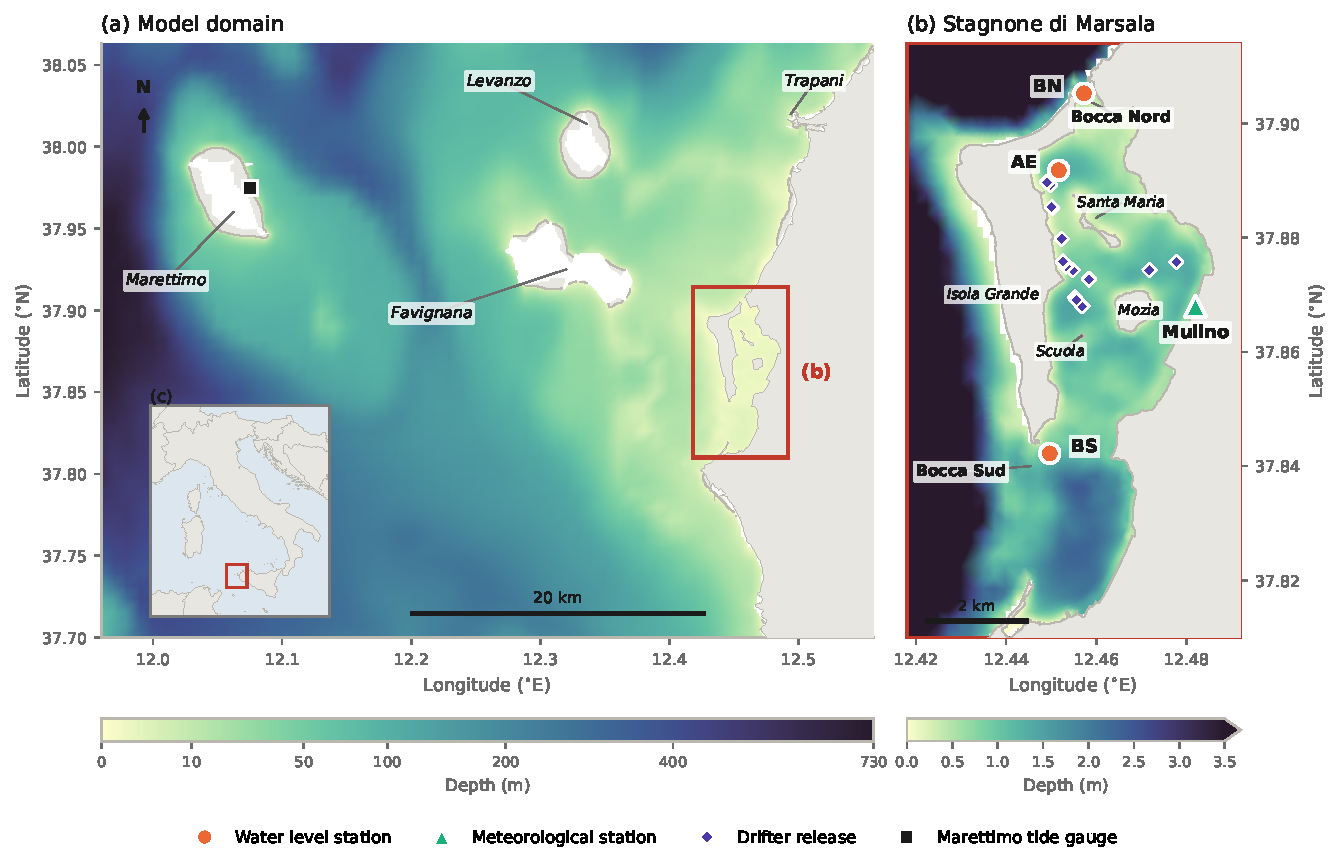
\includegraphics[width=\textwidth]{study_area_stagnone}
  \caption{The study area. (a) The modelled domain, covering western Sicily,
  the Egadi archipelago and the adjacent shelf, with the Marettimo tide gauge
  used for offshore validation. The red box gives the extent of panel (b).
  (b) The Stagnone di Marsala, with the water level stations (BocaNord,
  AltaVilaEst, BocaSud), the Mulino meteorological station, and the 35 GPS
  drifter release positions of the twelve July 2025 deployments.
  (c) The domain within Italy. Colour gives depth below the reference level on
  the model mesh, on separate scales for (a) and (b).}
  \label{fig:study_area}
\end{figure}

\section{Data and Methods}
\label{sec:data_methods}

\subsection{Hydrodynamic model}
\label{sec:methods_model}

Circulation was simulated with D-Flow Flexible Mesh (D-Flow FM, kernel
1.2.184) from the Delft3D FM Suite 2026.01, an unstructured finite-volume
solver for the three-dimensional shallow-water equations \citep{Kernkamp2011}.
The mesh of 25{,}212 faces covers the lagoon together with an offshore
extension reaching the western Sicilian channel, spanning 11.96--12.56$^\circ$E
and 37.70--38.06$^\circ$N, and grades from about 880~m offshore to about 60~m
in the lagoon and along the shorelines, so that about six cells span the 400~m
northern inlet. The vertical carries 10 sigma layers of uniform thickness,
about 0.095~m at the mean depth of 0.95~m, which resolves the wind-driven
surface drift over the near-bed return flow reported by \citet{DeMarchis2012}
and spreads the 0.40~m canopy of Section~\ref{sec:methods_roughness} over the
lowest four layers and part of the fifth.

Turbulence closure used the $k$--$\varepsilon$ model, and density followed the
UNESCO equation of state with salinity and temperature as active constituents,
so that the summer hypersaline gradient contributes baroclinically. Bed
roughness was a uniform Manning coefficient of 0.023~s~m$^{-1/3}$ in every
member, the default of the solver, which stands for the bare substrate and was
held uniform by design so that the canopy is the only spatially variable
resistance in the ensemble. Wind drag followed the Charnock formulation with
the coefficient taken from the ERA5 field. The simulation covered 1 to
10~July 2025 with an adaptive time step under a Courant limit of 0.7, capped at
30~s in the members coupled to the wave model and at 15~s in the uncoupled ones,
on eight MPI partitions. The numerical settings, their grounds and the run
times are given in the Supplementary Material, Section~S1.

\subsection{Wave model and coupling}
\label{sec:methods_waves}

Waves were computed with SWAN \citep{Booij1999} through the Delft3D-WAVE
module, on an outer grid of $69 \times 54$ points at about 800~m over the whole
domain and an inner grid at about 90 by 110~m over the lagoon and its inlets,
with third-generation physics, depth-induced breaking \citep{BattjesJanssen1978}
and JONSWAP bottom friction. Flow and waves exchanged fields every 3600~s
through the DIMR framework, an interval set by the tidal and sea-breeze time
scales the coupling has to resolve, and wave forces entered the flow as
three-dimensional dissipation. Within each exchange the wave model ran in
stationary mode, which holds because wave energy crosses the 2.5~km basin in
about fifteen minutes. The spectral discretisation, the source terms and the
ground for each setting are given in Section~S2 and Table~S1.

\subsection{Boundary and atmospheric forcing}
\label{sec:methods_forcing}

Open-sea boundaries were forced with the CMEMS Mediterranean Sea physical
reanalysis. Water level, salinity, and temperature were prescribed along the
offshore boundary, together with a depth-resolved advection velocity, which was
necessary for stability in the deep offshore cells, where a water-level-only
boundary admitted spurious accelerations. Since the CMEMS sea surface height is
an anomaly about the model rest state rather than a geodetic level, a per-node
offset of $+0.449$~m, anchored on the Marettimo tide gauge over 384 days and
distributed along the boundary by the CMEMS mean dynamic topography, was added
to the water-level boundary. Its seasonal residual of about 0.07~m bounds the
accuracy of the reference level the model can be held to (Section~S3).

Wind components, mean sea level pressure and the Charnock parameter were taken
from ERA5, the wind field blended with the record of the AltaVilaEst station,
and evaporation was imposed as negative rainfall. Interior salinity and
temperature were nudged towards the CMEMS fields with a relaxation time of
$8.64\times10^{5}$~s, long enough to leave the lagoon interior essentially
free-running while constraining the offshore extension.

Temperature and salinity outside the lagoon were initialised with the depth
profiles of the CMEMS nudging field at the start time, applied over the domain,
from 25.8~$^\circ$C and 37.5 at the surface to 16.2~$^\circ$C and 38.3 below
260~m. The hypersaline value of 42 was prescribed over the lagoon, whose
temperature takes the surface value of the profile.

\subsection{Seagrass canopy parametrisation}
\label{sec:methods_roughness}

The canopy was represented as a three-dimensional drag field, resolved per sigma
layer over the vertical extent the plants occupy. A cell whose canopy fills two
fifths of the water column carries drag in the layers within that fraction and
none above it. Drag per unit volume follows the standard quadratic form
\citep{Nepf2012}, with a drag coefficient $C_D$, a stem diameter $D$, an areal
stem density $m$ and a canopy height $h_v$.

The alternative available in this solver is the trachytope framework, in which
vegetation enters as a composite bed roughness following \citet{Baptist2007}.
It was not adopted here, since a roughness term acts at the bed whereas the
quantity the factorial has to separate is a momentum sink distributed through
the part of the column the plants occupy. For the same reason the calibrated
value of \citet{Ingrassia2024} for this lagoon, a Gauckler--Strickler
coefficient of 20~m$^{1/3}$~s$^{-1}$ equivalent to a Manning coefficient of
0.050~s~m$^{-1/3}$, is a bulk roughness of the vegetated basin, and used as the
bare-substrate roughness of a model that resolves the canopy it would count the
canopy twice.

Table~\ref{tab:veg} gives the values and their provenance. None was fitted to
any observation used to evaluate the model. Densities are expressed per leaf,
since it is the leaf that presents the frontal area, and the canopy height is
the deflected extent of the drag rather than the leaf length, taken within the
range of the flume and large-scale measurements of the species
(Section~S4). Fractional cover from the classification multiplies the areal
density and nothing else, height and diameter being properties of the plant
rather than of how much bed it covers, and median cover is 0.685 for
\emph{P.\ oceanica} and 0.181 for \emph{C.\ nodosa}, which therefore carries
about 1.5\% of the total canopy frontal area.

\begin{table}[H]
  \centering
  \caption{Canopy parameters. \emph{P.\ oceanica} values are from
  \citet{CiraoloFerreri2006}, except the canopy height, which is from
  \citet{Prinos2010}. \emph{C.\ nodosa} values are from \citet{Morris2008},
  with the shoot density also bracketed by \citet{Cancemi2002}.}
  \label{tab:veg}
  \begin{tabular}{lrr}
    \toprule
    Parameter & \emph{P.\ oceanica} & \emph{C.\ nodosa} \\
    \midrule
    Shoot density (m$^{-2}$)      & 500   & 800   \\
    Leaves per shoot              & 6     & 3     \\
    Leaf width $D$ (m)            & 0.010 & 0.004 \\
    Canopy height $h_v$ (m)       & 0.40  & 0.15  \\
    Leaf density (kg~m$^{-3}$)    & 900   & 900   \\
    Drag coefficient $C_D$        & 0.8   & 0.8   \\
    \bottomrule
  \end{tabular}
\end{table}

The spatial assignment of classes came from a supervised random-forest
classification of PlanetScope SuperDove imagery acquired in August 2023 at 3~m
ground sampling distance, following the depth-invariant approach of
\citet{Maltese2025}, and classified pixels were transferred to the flow links
of the mesh, a link straddling more than one class carrying each weighted by
the area it occupies (Figure~\ref{fig:seagrass}, Section~S4).

\begin{figure}[H]
  \centering
  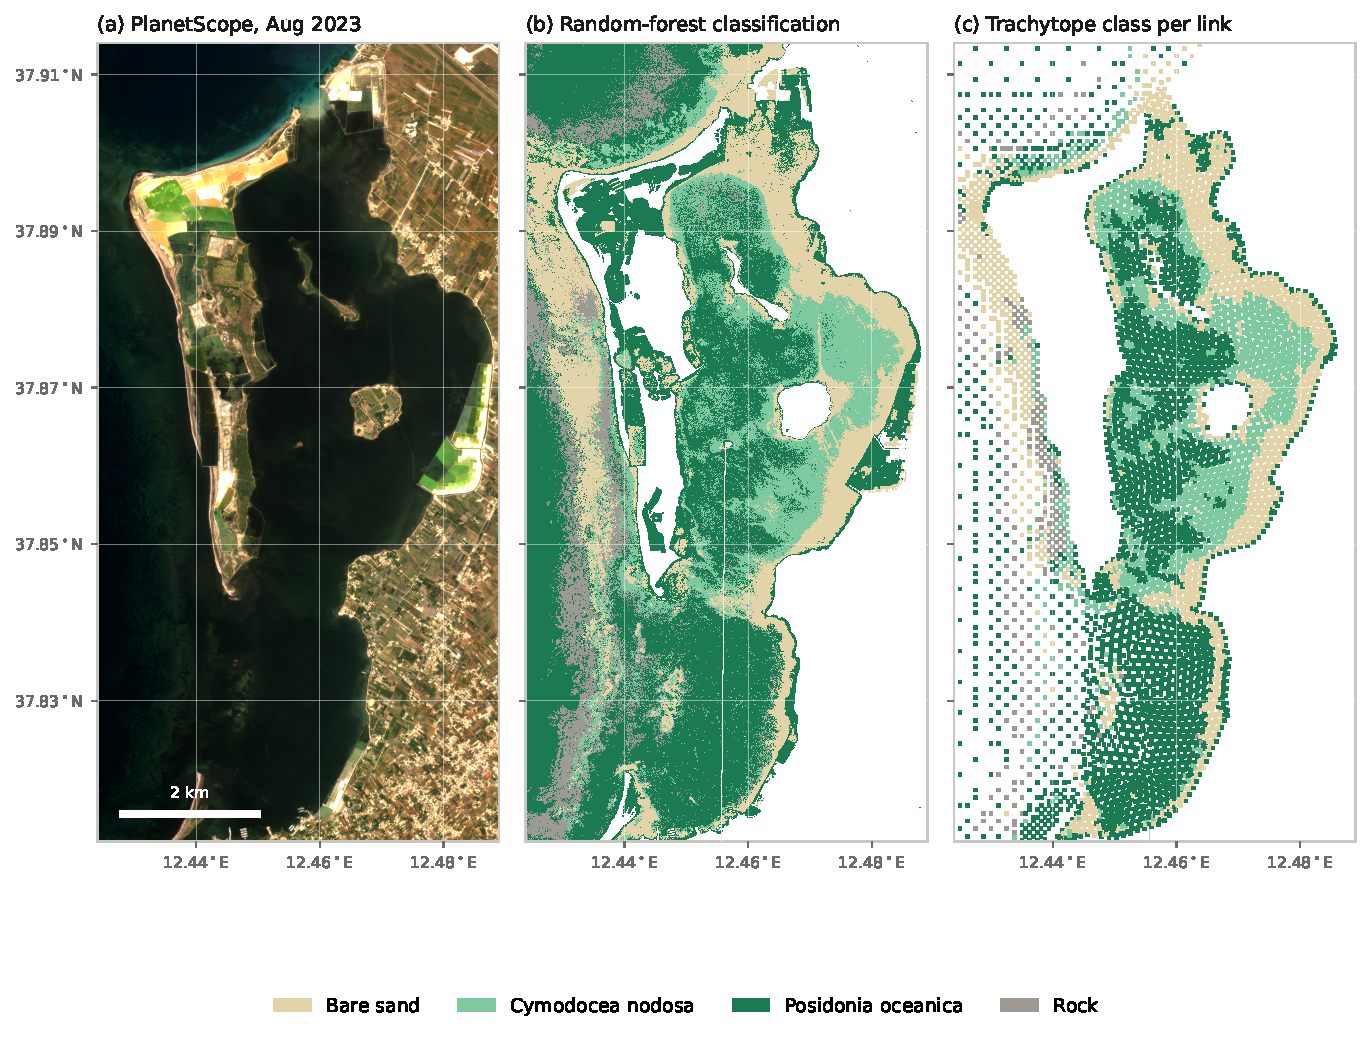
\includegraphics[width=\textwidth]{seagrass_classification}
  \caption{The seagrass map from imagery to model input. (a) PlanetScope
  SuperDove August 2023 median composite. (b) The random-forest classification,
  with the six output classes collapsed to the four seagrass classes.
  (c) The dominant class at each flow link, from the classification file
  the model reads, showing the mesh resolution the classification is sampled
  onto. The classification is computed over the whole scene, but only links
  inside the lagoon carry a canopy class.}
  \label{fig:seagrass}
\end{figure}

\subsection{Observational data and validation metrics}
\label{sec:methods_validation}

Water level was recorded at ten-minute resolution at three stations, BocaNord
at the northern inlet, BocaSud near the southern inlet, and AltaVilaEst on the
eastern flank of the central basin. Offshore performance was assessed at the
Marettimo tide gauge.

Water-level skill was quantified with the raw root-mean-square error, the
bias, and the anomaly root-mean-square error computed after removing the
respective means, together with the linear correlation and the ratio of
modelled to observed standard deviation. The three error measures are related
by $\mathrm{RMSE}^2 = \mathrm{bias}^2 + \mathrm{RMSE}_{\mathrm{anom}}^2$, so
reporting them jointly separates a constant reference-level offset from
genuine dynamic error in phase and amplitude. The first simulated day was
discarded as spin-up, over which the initial condition relaxes and the
transients it generates leave the basin.

Lagrangian skill was assessed against GPS-tracked surface drifters released in
the lagoon interior during the simulation window. Simulated trajectories were
obtained by advecting particles with OpenDrift \citep{Dagestad2018} through the
modelled surface current field, at an advection step of 300~s and with
positions written every 600~s. Scoring was restricted, for each drifter, to
the interval between its first and last observation, since the advection
continues to the end of the forcing while the deployments last between 0.4 and
7.2~h. A wind drift factor of 0.02 was applied to every member, since a sweep
over this parameter found no single value optimal across deployments and a
per-member value would have confounded the process attribution with a tuning
difference.

Agreement was quantified with the normalised cumulative
Lagrangian separation skill score of \citet{Liu2011}, which accumulates the
separation between modelled and observed positions and normalises it by the
distance travelled by the observed drifter, and with the endpoint proximity,
the separation between modelled and observed positions at the end of each
deployment. \citet{Revelard2021} discuss the sensitivity of this class of
metric to the normalisation choice in coastal applications.

\subsection{Numerical experiments}
\label{sec:methods_experiments}

Eight simulations were run over the same nine-day window, from the same initial
condition and with identical boundary and atmospheric forcing, so that the
differences between them isolate individual model components. All eight share
the mesh, and all wrote station output every 600~s and gridded output every
1800~s, so the comparison is not affected by differences in output sampling.

Members are identified by a three-slot code whose slots mark wave coupling,
seagrass canopy and mobile bed in that order, carrying \texttt{W}, \texttt{V}
or \texttt{M} where the factor is active and a dash where it is not. The eight
are \texttt{{-}{-}{-}}, \texttt{{-}V{-}}, \texttt{W{-}{-}}, \texttt{WV{-}},
\texttt{{-}{-}M}, \texttt{{-}VM}, \texttt{W{-}M} and \texttt{WVM}, and the code
is used throughout the results.

The design is a complete factorial in three factors, wave coupling, seagrass
canopy and bed mobility, and all eight cells were obtained. The process
attribution is made on the four fixed-bed members, a two-factor design in wave
coupling and canopy, and the four mobile-bed members form a sensitivity arm,
the critical shear stress for erosion not having been constrained against a
repeated bathymetric survey. Each vegetated member is a three-day segment
restarted on 7~July from the state of the bare member of the same cell, so the
two members of a pair share the first six days and differ by the canopy over
the window in which they are scored. In the mobile-bed members suspended
sediment does not contribute to the density field, and erodible sediment is
confined to depths above 15 to 20~m, where waves can plausibly move it
(Section~S5). The effect of the mobile bed on transport was traced with two
segments of the wave-coupled mobile-bed member without canopy, restarted on
7~July from its state on that date, one with the bed updated as in the member
and one with the bed held at that state.

The whole ensemble was also repeated from a vertically uniform column, at
24~$^\circ$C and 37.5 outside the lagoon and with the same hypersaline value
inside it. The horizontal and vertical resolution, a time-step limit by the
vertical fluxes, and the host and decomposition were tested on the uncoupled
fixed-bed configuration without canopy, as described in Section~S6.

\section{Results}
\label{sec:results}

All eight members are scored on a common interval, 8 to 10 July 2025, which is
the intersection of the members' post-spinup spans and which contains the whole
drifter record. Members are coded by wave coupling (W), seagrass canopy (V) and
mobile bed (M). The attribution rests on the four fixed-bed members, and the
mobile-bed arm is reported beside them in the tables and examined in
Section~\ref{sec:res_sensitivity}.

\subsection{Water level}
\label{sec:res_wl}

Table~\ref{tab:wl} reports water level skill at the three interior stations.
Raw error is dominated by a positive bias at BocaNord and AltaVilaEst, between
0.03 and 0.09~m, and by a negative one at BocaSud, between $-0.051$ and
$-0.015$~m. The bias is a datum and boundary-offset property that all members
share and it is not what distinguishes them.

The anomaly RMSE responds to different factors at the three stations
(Figure~\ref{fig:wl}b). At BocaSud it varies by 1.6~mm across the four
fixed-bed members. At BocaNord it varies by 12~mm and follows wave coupling,
falling from 0.039 to 0.027~m without a canopy and from 0.038 to 0.031~m with
one. At AltaVilaEst, the innermost station, in the northern basin where the meadow
is densest, it varies by 32~mm and follows the canopy, the two
vegetated members giving 0.021 and 0.028~m with correlations of 0.94 and 0.95
and the two bare members 0.048 and 0.054~m with correlations of 0.79 and 0.81.
Modelled-to-observed standard deviation ratios move the same way, from 1.18 and
1.37 without a canopy to 1.01 and 1.18 with one. The mobile-bed members
reproduce the values of their fixed-bed counterparts to within 3~mm, with one
exception, the bare wave-coupled member at AltaVilaEst, whose anomaly RMSE is
8~mm lower than on the fixed bed and remains 16~mm above that of its vegetated
counterpart.

The record itself shows where that error sits (Figure~\ref{fig:wl}a), with the
bare configurations overshooting the range of the observed anomaly and running
ahead of it, most visibly on the falling limb of 9 July, while the vegetated
ones track both the amplitude and the phase. The two arms are separated by more
than the spread within either of them over most of the window.

\begin{figure}[H]
  \centering
  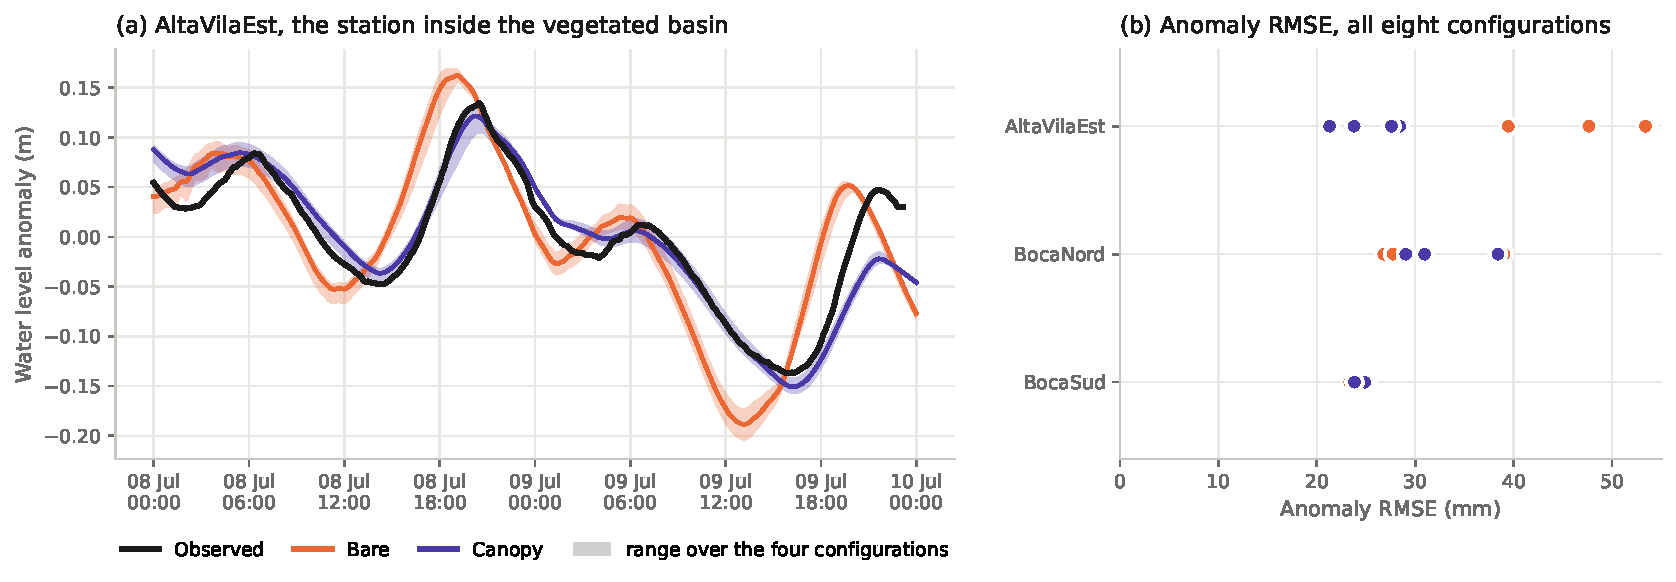
\includegraphics[width=\textwidth]{water_level_stations}
  \caption{Water level over the scored window. (a) Anomaly at AltaVilaEst,
  observed against the two arms, each drawn as its mean and the envelope of its
  four configurations, the mobile-bed ones included. Anomalies rather than raw
  levels, because the bias is common to all eight members. (b) Anomaly RMSE at
  the three stations for every configuration, coloured by canopy treatment.}
  \label{fig:wl}
\end{figure}

The vegetated members are three-day segments restarted from the bare member of
the same cell, and a segment run without any other change reproduces its
continuous member in water level and drifter skill (Supplementary Material,
Section~S7), so the separation at AltaVilaEst does not reflect the restart.

\begin{table}[H]
  \centering
  \caption{Water level skill by member and station, 8--10 July 2025.
  $\mathrm{RMSE}^2 = \mathrm{bias}^2 + \mathrm{RMSE}_{\mathrm{anom}}^2$. Members
  are coded by wave coupling (W), seagrass canopy (V) and mobile bed (M); the
  last four of each station form the mobile-bed arm. All values in metres
  except the dimensionless ratios.}
  \label{tab:wl}
  \begin{tabular}{llrrrrr}
    \toprule
    Station & Member & RMSE & Bias & RMSE$_{\mathrm{anom}}$ & $r$ & $\sigma_m/\sigma_o$ \\
    \midrule
    BocaNord & \texttt{{-}{-}{-}}  & 0.052 & $+0.035$ & 0.039 & 0.89 & 1.20 \\
             & \texttt{{-}V{-}}    & 0.050 & $+0.033$ & 0.038 & 0.90 & 1.22 \\
             & \texttt{W{-}{-}}    & 0.065 & $+0.059$ & 0.027 & 0.94 & 1.08 \\
             & \texttt{WV{-}}      & 0.059 & $+0.051$ & 0.031 & 0.92 & 1.09 \\
             & \texttt{{-}{-}M}    & 0.052 & $+0.034$ & 0.039 & 0.89 & 1.20 \\
             & \texttt{{-}VM}      & 0.050 & $+0.032$ & 0.038 & 0.90 & 1.22 \\
             & \texttt{W{-}M}      & 0.066 & $+0.060$ & 0.028 & 0.94 & 1.12 \\
             & \texttt{WVM}        & 0.059 & $+0.051$ & 0.029 & 0.94 & 1.15 \\
    \midrule
    BocaSud  & \texttt{{-}{-}{-}}  & 0.050 & $-0.043$ & 0.025 & 0.95 & 1.20 \\
             & \texttt{{-}V{-}}    & 0.057 & $-0.051$ & 0.025 & 0.95 & 1.16 \\
             & \texttt{W{-}{-}}    & 0.028 & $-0.015$ & 0.024 & 0.94 & 1.06 \\
             & \texttt{WV{-}}      & 0.035 & $-0.025$ & 0.025 & 0.93 & 1.02 \\
             & \texttt{{-}{-}M}    & 0.049 & $-0.043$ & 0.025 & 0.95 & 1.20 \\
             & \texttt{{-}VM}      & 0.057 & $-0.051$ & 0.025 & 0.95 & 1.16 \\
             & \texttt{W{-}M}      & 0.033 & $-0.023$ & 0.023 & 0.94 & 1.08 \\
             & \texttt{WVM}        & 0.037 & $-0.028$ & 0.024 & 0.93 & 1.05 \\
    \midrule
    AltaVila & \texttt{{-}{-}{-}}  & 0.076 & $+0.053$ & 0.054 & 0.81 & 1.37 \\
    Est      & \texttt{{-}V{-}}    & 0.049 & $+0.040$ & 0.028 & 0.94 & 1.18 \\
             & \texttt{W{-}{-}}    & 0.097 & $+0.085$ & 0.048 & 0.79 & 1.18 \\
             & \texttt{WV{-}}      & 0.070 & $+0.067$ & 0.021 & 0.95 & 1.01 \\
             & \texttt{{-}{-}M}    & 0.077 & $+0.055$ & 0.053 & 0.81 & 1.36 \\
             & \texttt{{-}VM}      & 0.050 & $+0.042$ & 0.028 & 0.94 & 1.17 \\
             & \texttt{W{-}M}      & 0.074 & $+0.062$ & 0.040 & 0.86 & 1.19 \\
             & \texttt{WVM}        & 0.062 & $+0.057$ & 0.024 & 0.94 & 1.01 \\
      \bottomrule
  \end{tabular}
\end{table}

\subsection{Lagrangian transport}
\label{sec:res_drifters}

Thirty-five drifters across twelve deployments were scored against each member
over the interval each drifter was in the water, which ranged from 0.4 to
7.2~hours. Table~\ref{tab:lagrangian} summarises the metrics and
Figure~\ref{fig:lagrangian} shows their distribution.

On the fixed bed, mean Liu--Weisberg skill spans 0.597 to 0.739 and endpoint
separation 327 to 481~m, and the four members divide cleanly on the canopy. The
two vegetated members score 0.711 and 0.739 and the two bare ones 0.597 and
0.619, and the two pairs do not overlap. The two components of the trajectory
error move together and both improve with the canopy, path length ratio rising
from 0.80 and 0.83 without a canopy to 0.88 and 0.94 with one, and mean heading
error falling from 11.2 and 10.4$^\circ$ to 8.5 and 8.4$^\circ$.

\begin{table}[H]
  \centering
  \caption{Lagrangian metrics by ensemble member, 35 drifters over twelve
  deployments, scored on the interval each drifter was in the water. Path ratio
  is simulated over observed path length. Heading error is the mean angular
  difference between simulated and observed step directions and is computed on
  eleven deployments, deployment 4 having too few positions to form the three
  step bearings it requires. The lower block is the mobile-bed arm
  (Section~\ref{sec:res_sensitivity}).}
  \label{tab:lagrangian}
  \begin{tabular}{lccrrrr}
    \toprule
    Member & Waves & Canopy & LW skill & Endpoint (m) & Path & Heading \\
    \midrule
    \texttt{{-}{-}{-}} & no  & no  & 0.619 & 478 & 0.80 & 11.2$^\circ$ \\
    \texttt{{-}V{-}}   & no  & yes & \textbf{0.739} & \textbf{327} & 0.88 & 8.5$^\circ$ \\
    \texttt{W{-}{-}}   & yes & no  & 0.597 & 481 & 0.83 & 10.4$^\circ$ \\
    \texttt{WV{-}}     & yes & yes & 0.711 & 335 & \textbf{0.94} & \textbf{8.4}$^\circ$ \\
    \midrule
    \multicolumn{7}{l}{\textit{Mobile bed}} \\
    \texttt{{-}{-}M}   & no  & no  & 0.614 & 479 & 0.80 & 11.4$^\circ$ \\
    \texttt{{-}VM}     & no  & yes & 0.739 & 330 & 0.88 & 8.5$^\circ$ \\
    \texttt{W{-}M}     & yes & no  & 0.708 & 304 & 0.89 & 7.9$^\circ$ \\
    \texttt{WVM}       & yes & yes & 0.718 & 307 & 0.88 & 8.0$^\circ$ \\
    \bottomrule
  \end{tabular}
\end{table}

\begin{figure}[H]
  \centering
  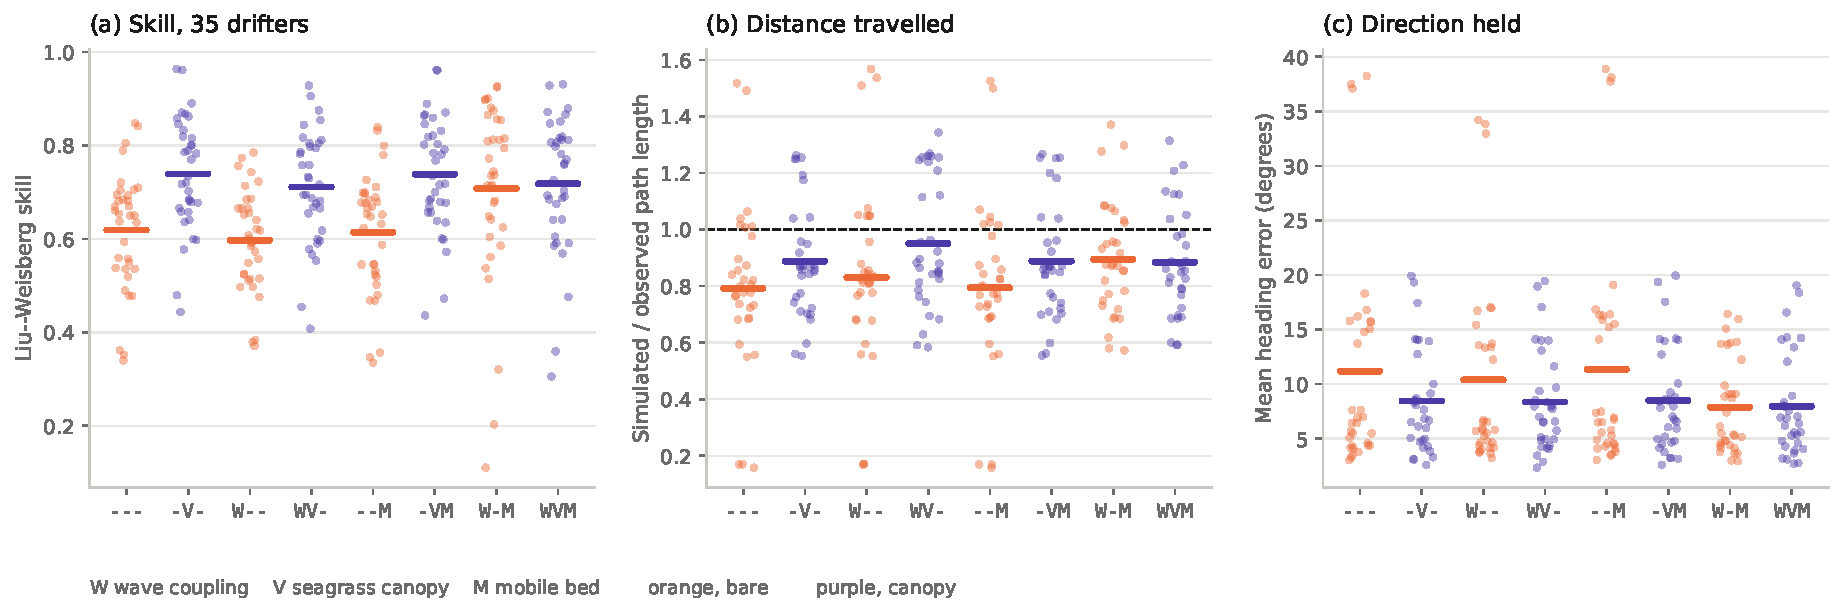
\includegraphics[width=\textwidth]{lagrangian_results}
  \caption{Lagrangian validation, one point per drifter and the bar giving the
  mean, the four fixed-bed members on the left and the mobile-bed arm on the
  right. (a) Liu--Weisberg skill. (b) Simulated over observed path length, the
  dashed line marking equality. (c) Mean angular difference between simulated
  and observed step directions. Panels (b) and (c) carry 32 drifters rather than
  35, deployment 4 having too few positions to form step bearings.}
  \label{fig:lagrangian}
\end{figure}

Figure~\ref{fig:tracks} shows the tracks for every deployment and for the
wave-coupled fixed-bed pair that differs only in the canopy. In the central
basin the bare particles leave the observed path early and finish short of the
observed endpoint while the vegetated ones hold its heading, and in the
southern deployments both follow the observed path closely, deployment 4 being
the exception.

\begin{figure}[H]
  \centering
  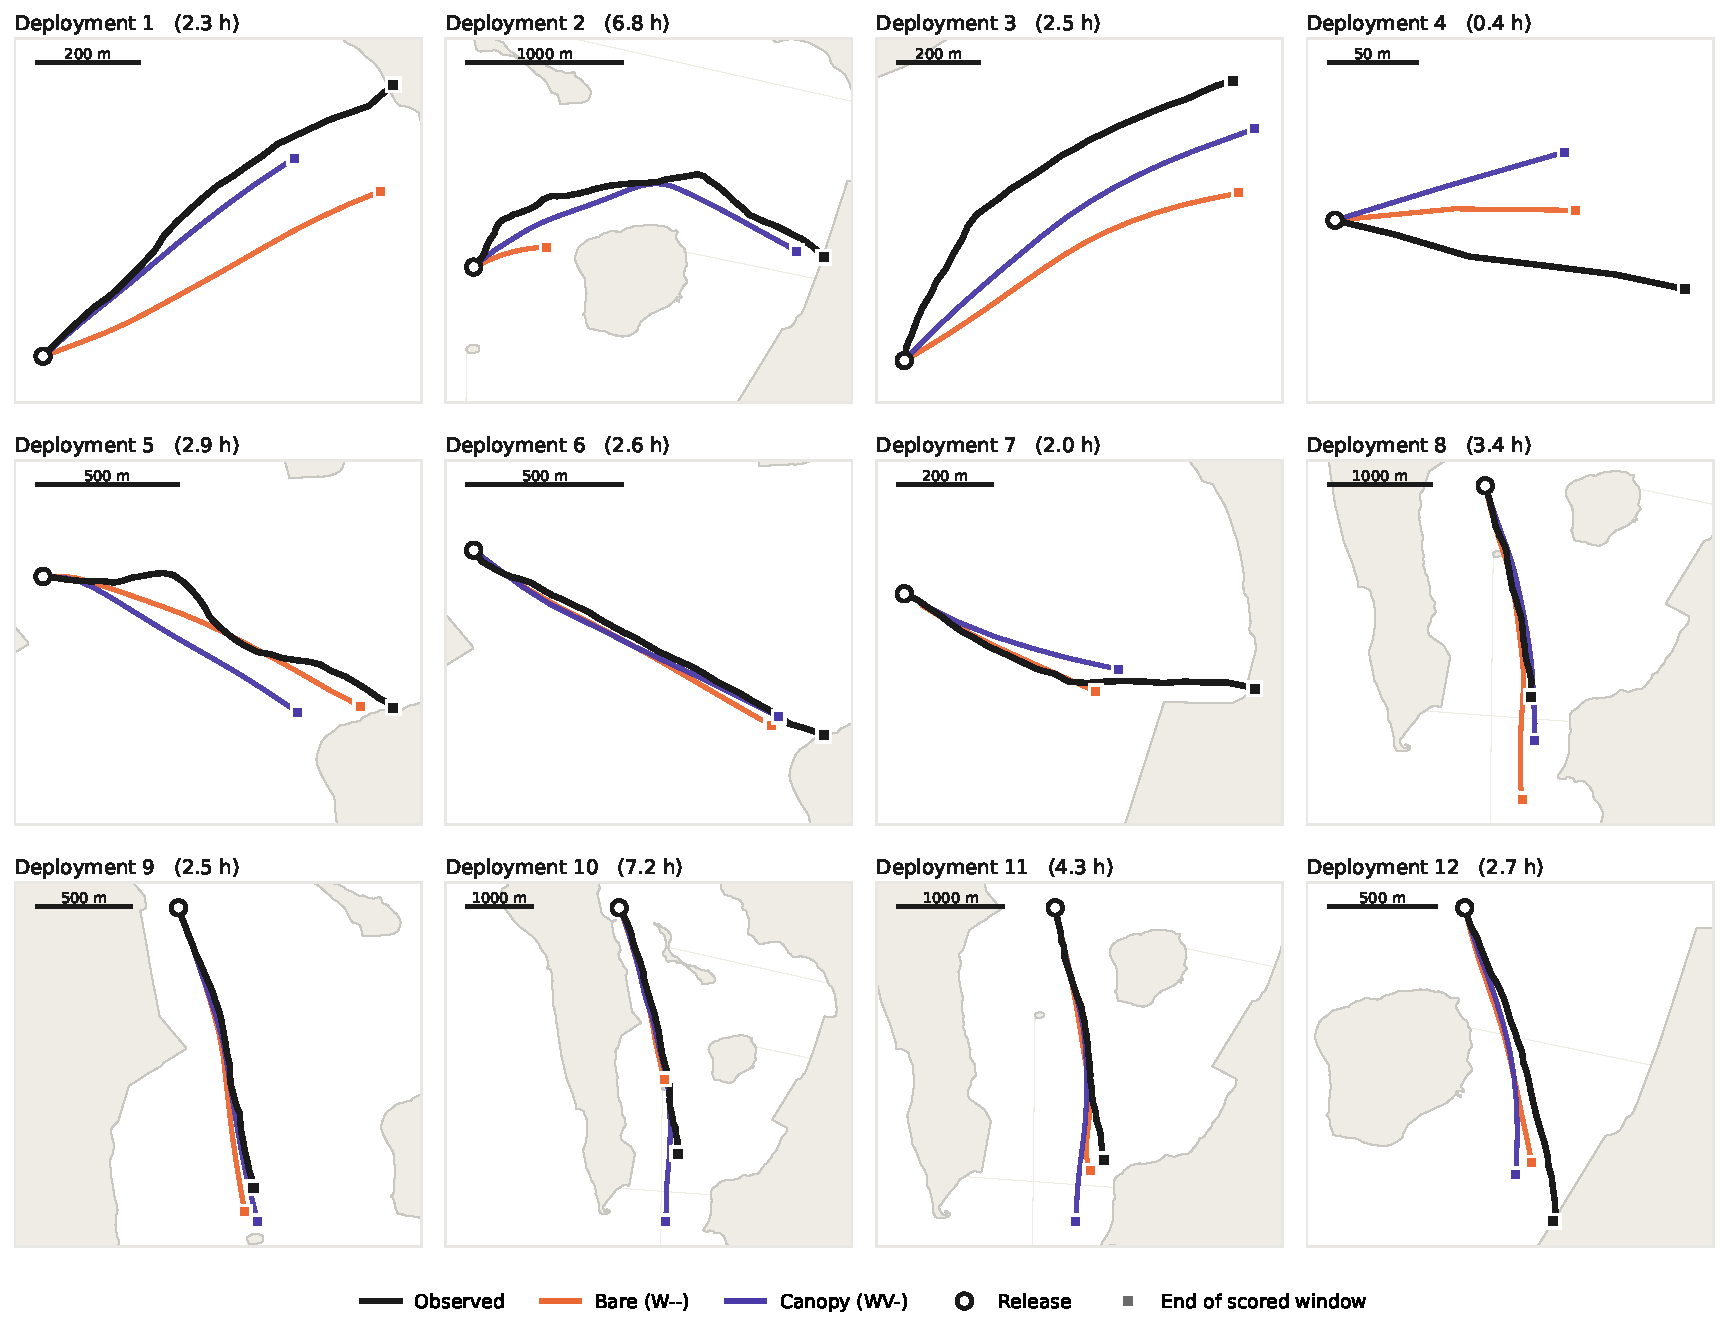
\includegraphics[width=\textwidth]{drifter_trajectories}
  \caption{Observed and simulated drifter trajectories, all twelve deployments,
  for the wave-coupled fixed-bed configurations that differ only in the canopy.
  One drifter per panel, the median-skill drifter of its deployment under the
  vegetated configuration. Circles mark the release and squares the end of the
  scored window. Each track is clipped to the interval its drifter was in the
  water. Panel extents differ, so each carries its own scale bar.}
  \label{fig:tracks}
\end{figure}

\subsection{Process attribution}
\label{sec:res_attribution}

On the fixed bed the design is a two-factor factorial in wave coupling and
canopy, with two single-factor contrasts per factor.
Figure~\ref{fig:attribution} gives them, with the contrasts that involve the
mobile bed beside them, with bootstrap confidence intervals over 4000 paired
resamples.

\textbf{Canopy.} The canopy raises skill by 0.120 (95\% CI $+0.061$ to $+0.180$)
without waves and by 0.114 (CI $+0.056$ to $+0.170$) with them, with 25 and 27
of the 35 drifters improving. Both intervals are clear of zero, and the two
contrasts agree to within 0.006, so the canopy effect does not depend on the
wave treatment.

\textbf{Wave coupling.} Wave coupling reduces skill by 0.022 (CI $-0.043$ to
$-0.003$) without a canopy and by 0.028 (CI $-0.040$ to $-0.017$) with one,
with 21 and 25 of the 35 drifters worse. The effect is a fifth of that of the
canopy, and the interaction term of the two factors is $-0.006$.

The canopy contrast holds deployment by deployment (Figure~\ref{fig:attribution}b),
with the same sign under both wave treatments in ten of the twelve deployments.
Deployment 4, the shortest record and the one deployment in which the bare
members score higher, is retained, and excluding it widens the two canopy
contrasts to $+0.148$ and $+0.144$ (Section~S7).

\begin{figure}[H]
  \centering
  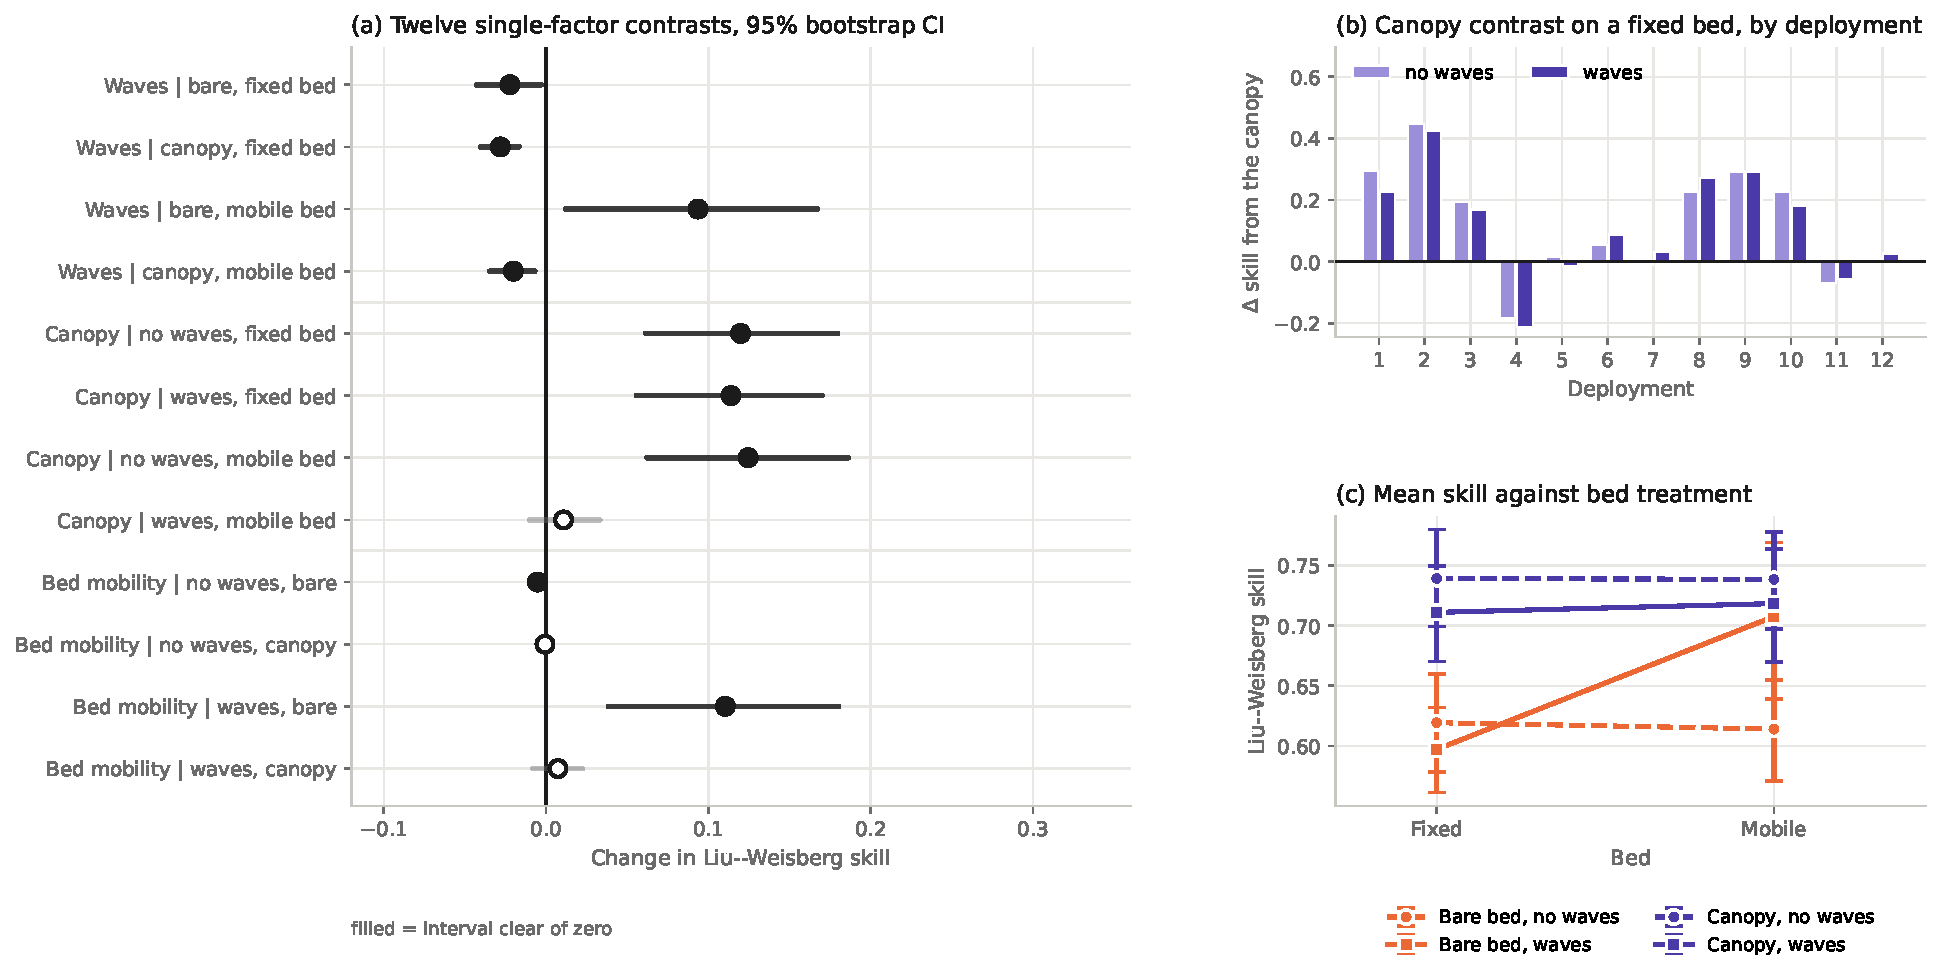
\includegraphics[width=\textwidth]{ensemble_attribution}
  \caption{Process attribution. (a) The twelve single-factor contrasts of the
  three-factor design with 95\% bootstrap intervals over 4000 paired resamples,
  filled markers denoting intervals clear of zero; the contrasts involving the
  mobile bed belong to the sensitivity arm. (b) The canopy contrast on the
  fixed bed, deployment by deployment, without and with wave coupling. (c) Mean
  skill against bed treatment, one line per combination of canopy and wave
  treatment, with 95\% intervals on each mean.}
  \label{fig:attribution}
\end{figure}

\subsection{Three-dimensional structure}
\label{sec:res_3d}

Over the wet cells of the lagoon interior, with the inlets excluded, mean
current speed increases monotonically from the bed to the surface in every
member (Figure~\ref{fig:profile}), and the canopy sets the shape of that
profile. On the fixed bed without a canopy, bed-layer speed is 0.032 to
0.035~\si{\metre\per\second} and surface-layer speed 0.065 to
0.069~\si{\metre\per\second}, for surface-to-bed ratios of 1.88 and 2.14. With a
canopy, bed-layer speed falls to 0.0093 to 0.0095~\si{\metre\per\second} while
surface speed falls much less, to 0.043 to 0.047~\si{\metre\per\second}, and the
ratio rises to 4.50 and 5.05.

Wave coupling moves the ratio by far less, adding 0.26 in the bare arm and 0.55
in the vegetated one, against a canopy contribution of $+2.62$ without waves and
$+2.91$ with them.

Bed shear stress separates the two treatments by sign rather than by magnitude.
Averaged over the meadow on 8 July in members started from the stratified
column, as the ensemble is, it fell from 0.028 to 0.0026~\si{\pascal} when the
canopy was introduced, a factor of 11, while a member representing the same
meadow as an equivalent bed roughness instead of as a canopy raised it to
0.043~\si{\pascal} over the same cells and times.

Lagoon-mean surface speed does not order the members the way transport does,
since the member reproducing the observed drifter behaviour best has the lowest
lagoon-mean surface speed of the fixed-bed members at
0.043~\si{\metre\per\second}, against 0.069 for a member whose particles travel
17\% too short a distance.

\begin{figure}[H]
  \centering
  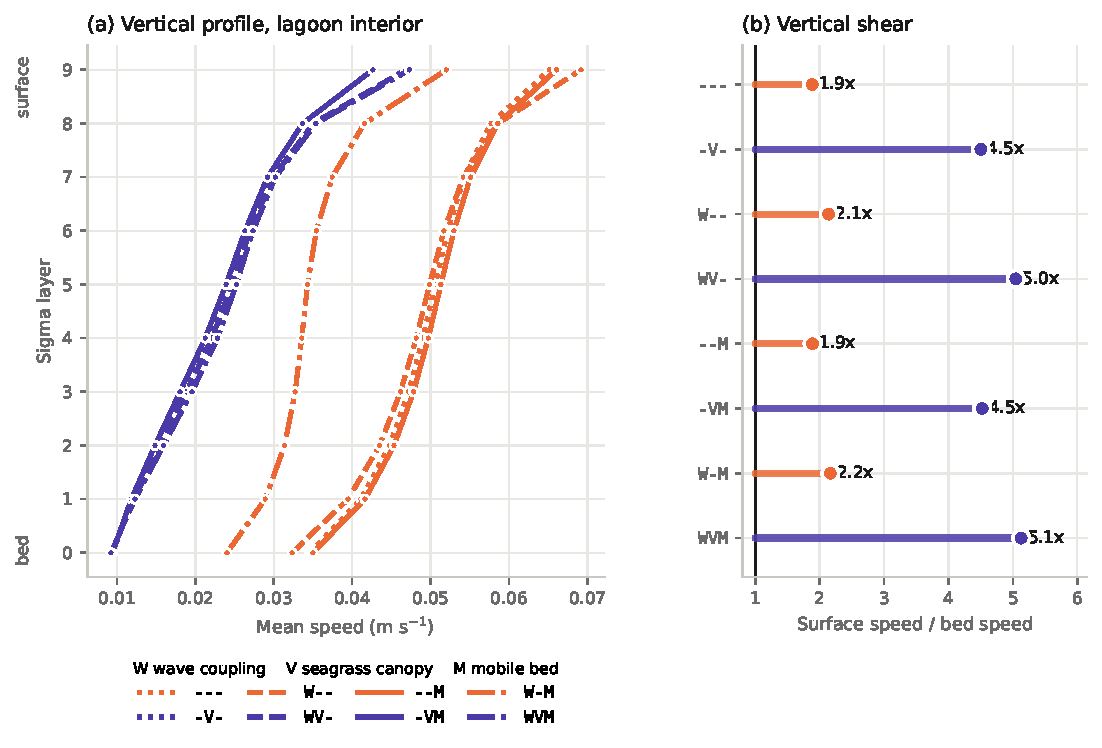
\includegraphics[width=0.88\textwidth]{layer_profile_lagoon}
  \caption{Vertical structure in the lagoon interior over the drifter window.
  (a) Mean speed by sigma layer, colour giving the canopy treatment and line
  style the wave and bed treatments. (b) The ratio of surface to bed speed.}
  \label{fig:profile}
\end{figure}

\subsection{Response of the seagrass classes}
\label{sec:res_classes}

Cells were grouped by the seagrass class of the nearest classified point. The
classes occupy different parts of the basin at different depths, and the bare
fixed-bed configurations already have their \emph{Posidonia} cells slower at
the bed than their sand cells, in a ratio of 0.91 and 0.92, so the canopy
effect is read between configurations within a class or as a change in that
ratio.

Under either reading the effect is large and correctly ordered, since on the
fixed bed introducing the canopy reduces mean bed speed by 78\% over
\emph{Posidonia} and 77\% over \emph{Cymodocea}, against 59\% over sand and 57\%
over rock (Figure~\ref{fig:classes}b). The \emph{Posidonia} to sand bed-speed
ratio falls from 0.91 and 0.92 without a canopy to 0.49 with one, under both
wave treatments. The two unvegetated classes respond as well, because slowing
the flow through the meadow changes the circulation of a basin whose interior
is largely meadow, but they respond by a quarter less.

The canopy also removes most of the dependence on wave coupling, since within a
class mean bed speed differs between the two bare fixed-bed configurations by
0.002 to 0.010~\si{\metre\per\second} and between the two vegetated ones by
0.0002 to 0.0011~\si{\metre\per\second}. Once the canopy is present the near-bed
flow is nearly the same whatever the wave treatment, which is the near-bed
counterpart of the agreement in transport skill reported in
Section~\ref{sec:res_drifters}.

The wave field does not follow the flow, mean orbital velocity at the bed
changing by 0.2 to 0.9\% over the four classes when the canopy is introduced on
the fixed bed (Figure~\ref{fig:classes}c), since the canopy does not reach the
wave computation (Section~\ref{sec:disc_limits}).

\begin{figure}[H]
  \centering
  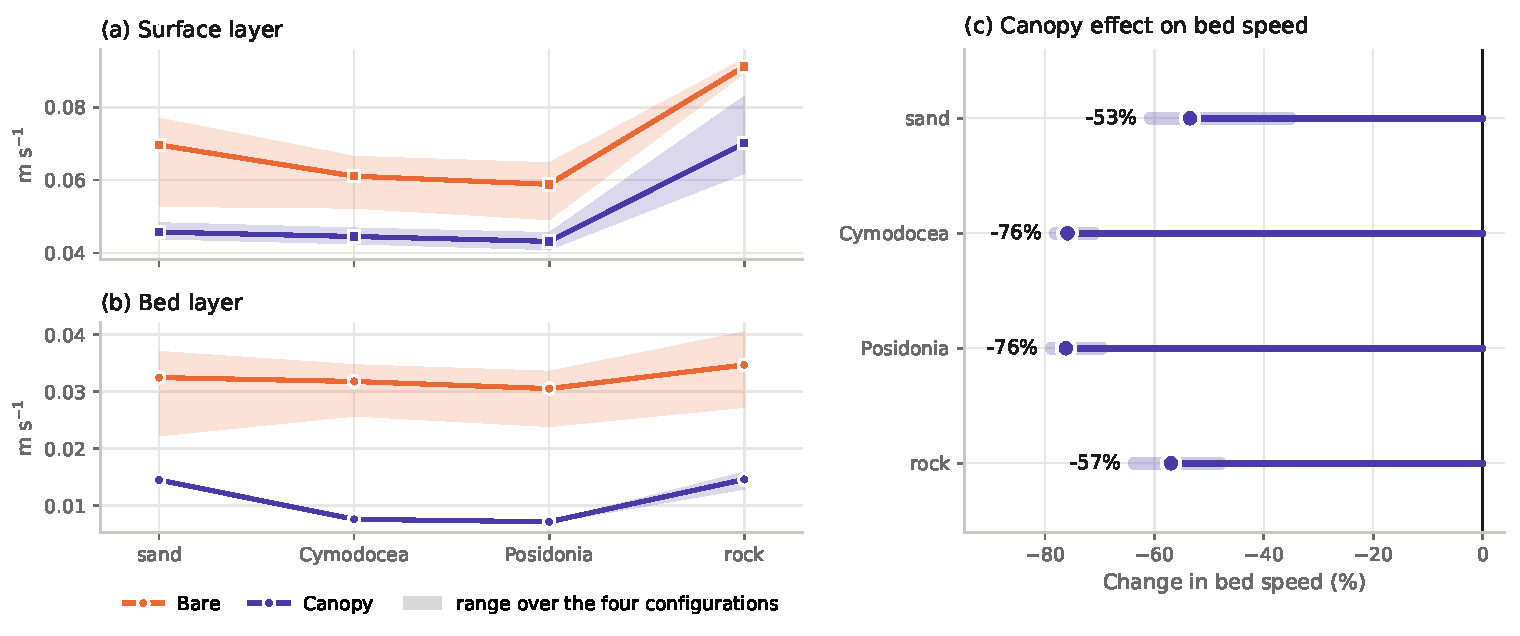
\includegraphics[width=\textwidth]{class_speed_uorb}
  \caption{Flow response by seagrass class in the lagoon interior. (a) Mean
  speed in the surface layer and (b) in the bed layer, the line giving the mean
  over the four configurations of each arm, the mobile-bed ones included, and
  the band their range. (c) Change in mean bed speed on introducing the canopy,
  the marker giving the mean over the four cells of the design and the band
  their range.}
  \label{fig:classes}
\end{figure}

\subsection{Sensitivity to bed mobility, initial condition and discretisation}
\label{sec:res_sensitivity}
\label{sec:res_numerics}

With wave coupling the mobile bed leaves any plausible state of the basin.
Averaged over the lagoon from 7 to 10 July, suspended sediment reaches
9.3~\si{\gram\per\litre} in the bare wave-coupled member and
9.4~\si{\gram\per\litre} in its vegetated counterpart, against 0.1 and
0.007~\si{\gram\per\litre} in the two uncoupled mobile-bed members, and the bed
of the lagoon loses 4.0 and 3.1~million~\si{\metre\cubed} over the nine days.
By 10 July the bare wave-coupled member has lowered the lagoon bed by 12~cm on
average and changed it by more than 5~cm over 74\% of its area, whereas without
waves the change exceeds 5~cm over 0.3\% of the area. The canopy does not
shield the bed from this erosion, because it does not reach the wave model.

The same bare member nevertheless scores 0.708 (Table~\ref{tab:lagrangian}),
close to the vegetated members, so that in the cell combining waves and a
mobile bed the canopy contrast falls to $+0.011$ (CI $-0.010$ to $+0.033$) and
the wave and bed-mobility contrasts of the bare arm reach $+0.094$ and $+0.111$
(Figure~\ref{fig:attribution}a). The two segments restarted on 7~July locate
the source of that skill. With the bed updated the segment scores 0.710 and
with the bed held at its 7~July state 0.707, a difference of $-0.003 \pm
0.004$, while the held bed scores $0.110 \pm 0.039$ above the fixed-bed member
\texttt{W{-}{-}}, with 29 of 35 drifters better. The gain therefore comes from
the bathymetry reshaped over the first six days and not from sediment transport
in the drifter window. At AltaVilaEst the member keeps an anomaly RMSE of
0.040~m and a correlation of 0.86, against 0.024~m and 0.94 for its vegetated
counterpart.

Started from a vertically uniform column instead of the stratified state, the
bare members score 0.080 to 0.145 lower and the vegetated members 0.005 to
0.018 lower, so that the canopy contrasts on the fixed bed become $+0.195$ and
$+0.188$. The uniform start raises the modelled mean water level at the gauges
by 2 to 10~cm and, on the fixed bed, changes anomaly RMSE by at most 4~mm and
correlation by at most 0.03, and the canopy signature at AltaVilaEst is the same
under both starts.

The horizontal and vertical resolution, the time-step limit and the host and
decomposition change skill by less than 0.01 under a Courant limit of 0.5 and
water level by at most 2.4~mm, so they do not limit the quantities the study
reports (Section~S6). Under the Courant limit of 0.7 used by the ensemble the
uncoupled member scores $0.034 \pm 0.004$ lower on four partitions on a second
computer than on eight on the server, a dependence that all members share.


\section{Discussion}
\label{sec:discussion}

\subsection{Vertical placement of the canopy drag}

This study asked which modelled processes control transport in a shallow
vegetated lagoon, and on the fixed bed the answer the ensemble gives is the
seagrass canopy, with an effect five times that of wave coupling and the same
under both wave treatments. The mechanism the model offers for that is vertical
rather than frictional, since introducing the canopy removes momentum from the
lower part of the water column without removing a proportionate amount from the
upper part, more than doubling the ratio of surface to bed speed. Such a profile
is the signature of a canopy shear layer rather than of a rougher bed, which
acts through a logarithmic profile whose surface-to-bed ratio is bounded well
below the value obtained here \citep{Nepf2012}, and the bed shear stress
confirms the distinction by its sign, falling under the canopy where an
equivalent bed roughness raises it over the same cells. Since a surface drifter
samples the top of that profile, a treatment that reshapes the profile relocates
the drifter even where it changes the depth-averaged transport little.

That places the present result in a particular relation to the two earlier
models of this basin rather than in opposition to them.
\citet{Ingrassia2024} obtained a best-fit uniform Gauckler--Strickler
coefficient for the vegetated lagoon within a depth-averaged framework, where an
equivalent bed roughness is the appropriate representation of a canopy because
there is no vertical profile for the canopy to shape. \citet{DeMarchis2012}
worked in three dimensions and assigned Nikuradse roughness heights by seagrass
class, establishing the vertical structure of the wind- and tide-driven
circulation that motivates using a three-dimensional solver here at all. Both
answered the questions they set, and a roughness representation reproduces the
drag the meadow exerts. What has changed since is the availability of a
canopy formulation that resolves that drag over the vertical extent the plants
occupy, and the contribution of the present work is to quantify what that
capability buys in a basin of this depth. The canopy parameters used here were
taken from published measurement of the two species and were not adjusted
against any observation, so the improvement follows from where the drag is
applied rather than from how it was tuned.

\subsection{Information carried by each gauge position}

Water level separated the configurations by the canopy at AltaVilaEst, by wave
coupling at BocaNord and by neither at BocaSud, and the three positions
constrain different parts of the problem. Agreement at the inlet gauges
establishes that the offshore forcing, the datum and the exchange through the
two mouths are right, and in a micro-tidal basin with two open connections those
set most of the level there, the wave contribution to the northern inlet being
the one dynamic effect that reaches it. Agreement in the interior tests
something the outer pair cannot, because the level there is set by what the
water does on its way in, which is where the canopy acts. The roles are
complementary, and a match in the interior would be difficult to interpret
without the exchange having been established first.

Together with the drifter result, the gauge result refines the familiar argument
that water level constrains transport weakly and that Lagrangian observations
form a distinct constraint rather than a confirmation \citep{Liu2011,
Revelard2021}. Water level is not inherently insensitive to the canopy, since
the one gauge sited inside the vegetated basin identified the same factor as the
drifters and ranked the fixed-bed configurations the same way. For a basin of
this type the useful question is therefore less whether to validate on water
level than where to place the instrument intended to discriminate, and the
interior of the vegetated compartment is a considerably more informative
position for that purpose than the inlet. Section~\ref{sec:disc_synergy} shows
that the interior gauge also discriminates where the drifters do not.

\subsection{Bare-bed skill through a reshaped bathymetry}
\label{sec:disc_synergy}

The mobile-bed arm contains one configuration that, taken on its own, supports
a strong statement about process coupling. In the bare arm, wave coupling and
bed mobility each leave Lagrangian skill nearly unchanged or lower it when
applied alone and raise it when applied together, with an interaction term of
$+0.116$, tight bootstrap intervals and a mechanism available in the literature,
since wave orbital motion sets the bed stress that mobilises sediment and
wave--tide coupling is known to govern the sediment dynamics of shallow
micro-tidal basins \citep{Carniello2011}. The combination brings the bare
member to 0.708, within 0.03 of the vegetated members, and removes the canopy
contrast in that cell.

The segments restarted on 7~July show that the statement has no physical basis
in this model. The skill is carried by the bathymetry that six days of
wave-driven erosion reshaped, through a lagoon holding near
9~\si{\gram\per\litre} of suspended sediment and losing 4~million~\si{\metre\cubed}
of bed in nine days, a state the basin does not reach in summer. The reshaped
bed does not reproduce the vertical structure of the canopy either, the
surface-to-bed speed ratio of that member remaining at 2.17 against 5.13 with
the canopy, so the agreement in skill is reached through a different flow. A
model without a canopy can therefore reach the drifter skill of a model with
one through a mechanism that is wrong, and the drifters alone do not separate
the two. The interior gauge does, since at AltaVilaEst the bare member keeps an
anomaly RMSE of 0.040~m and a correlation of 0.86 against 0.024~m and 0.94 for
its vegetated counterpart.

The initial condition shows the same asymmetry by another route. A start from a
uniform offshore column lowers the skill of the bare members by 0.08 to 0.15 and
that of the vegetated members by at most 0.02, so the canopy contrast grows from
about 0.12 to about 0.19 when the start is wrong. In both cases an error
elsewhere in the model degrades the bare configurations and leaves the
vegetated ones nearly unaffected, and the magnitude of a canopy contrast
therefore depends on what else the model gets wrong, even where its sign does
not.

What follows from this bears on how such an ensemble is read rather than on this
basin alone, since canopy drag is commonly left out of lagoon and estuary models
or folded into a bed roughness coefficient, and an ensemble built that way can
still return a well-defined and statistically clean interaction between the
processes it does carry. Here that interaction is produced by an implausible
morphodynamic state, and nothing internal to the bare half of the design
distinguishes it from a physical result. What distinguished them was varying
the canopy as a factor in its own right, checking the morphodynamic state
against a plausible sediment budget, and scoring the result against two
observation types that no model decision had used.

\subsection{Limitations}
\label{sec:disc_limits}

\textbf{Wave dissipation by the canopy.} The canopy does not reach the wave
model, because the coupling passes a bed roughness field to the spectral model
while the canopy enters the momentum equation of the flow, so mean orbital
velocity at the bed changes by under 1\% when the canopy is introduced and not
in an order that follows canopy density. Seagrass meadows do attenuate waves, in
this species and at this scale \citep{Infantes2012, Prinos2010}, and shallow
restricted Mediterranean lagoons carry wave fields that respond to bed
conditions \citep{Morote2025}. The wave field in these simulations is therefore
that of a bare bed, the wave contrasts reported here are conditional on that,
and so is the wave-driven erosion that the canopy fails to shield in the
mobile-bed arm. Representing canopy dissipation inside the spectral model is the
corresponding extension. It would be expected to change the wave contrasts
rather than the canopy ones, which are measured on the flow.

\textbf{Canopy reconfiguration.} The canopy bends under load rather than holding
a fixed height, and the response is dynamic, the velocity ratio between two
probes differing only in leaf stiffness moving from 1.005 in the slowest
quintile of the record to 0.807 in the fastest 5\%, where a fixed shortening
would give a constant ratio. A 13\% change in leaf density moves the velocity
field by 20\% at the upper end of the range, which is a strong sensitivity to a
value taken from a published table rather than measured in this meadow. The
bending is moreover mechanical, whereas the flume measurements of
\citet{CiraoloFerreri2006} describe reconfiguration empirically through a
friction factor that varies by a factor of twelve over the velocity range they
tested. That empirical formulation is available in the model only in its
depth-averaged solver, so the two could not be compared directly and the
agreement between them was not tested.

\textbf{Bed mobility.} The morphodynamic arm is not calibrated, the critical
shear stress for erosion having been constrained by neither a repeated
bathymetric survey nor a turbidity record, and with waves it leaves any
plausible state of the basin, with suspended sediment near
9~\si{\gram\per\litre} and the lagoon bed lowered by 12~cm on average in nine
days (Section~\ref{sec:res_sensitivity}). It is therefore a sensitivity test and
is kept out of the attribution. Before it could enter it, the erosion
parameters would need to bring suspended sediment in the lagoon to the order of
tens of milligrams per litre.

\textbf{Window and restart segments.} The record covers two days of water level
and thirty-four hours of drifter observations within one summer season, and the
vegetated configurations are three-day restart segments. A segment run without
any other change reproduces its continuous member in water level and drifter
skill (Section~\ref{sec:res_wl}), but seasonal behaviour, storm conditions and
the interaction of a canopy with a mobile bed over longer periods are outside
what this design addresses.

\textbf{Initial condition.} The ensemble starts from the depth profiles of the
CMEMS field at the start time, which a start from a uniform column does not
approach within the nine days, and from the uniform start the canopy contrasts
on the fixed bed are $+0.195$ and $+0.188$ rather than $+0.120$ and $+0.114$
(Section~\ref{sec:res_sensitivity}). The stratified start is itself a single
profile applied over the domain and leaves out the horizontal structure of the
CMEMS field, so the canopy contrasts reported here may still carry part of a
start-up adjustment. The solution also depends on the host and the
decomposition at the Courant limit of the ensemble, by 0.034 in skill from the
uniform start, which all members share, while the horizontal and vertical
resolution do not limit the reported quantities.

\textbf{\emph{Cymodocea nodosa} parameters.} The \emph{C.\ nodosa} parameters
are loosely constrained, coming from a flume study of plants collected
elsewhere, since no measurement of that species in this lagoon was available.
The species carries about 1.5\% of the canopy frontal area in the model, which
bounds the consequence, and the drag is carried almost entirely by the
\emph{P.\ oceanica} column.

\section{Conclusions}
\label{sec:conclusions}

In a shallow Mediterranean lagoon where the seagrass canopy occupies most of the
basin and the mean depth is below one metre, the canopy emerges from this
ensemble as the first-order control on Lagrangian transport. On the fixed bed,
representing it raises Liu--Weisberg skill by 0.120 without wave coupling and by
0.114 with it, both bootstrap intervals clear of zero, against $-0.022$ and
$-0.028$ for wave coupling, and the two factors do not interact.

The results indicate that where the drag is applied matters more than how it is
calibrated. The canopy here is a three-dimensional drag field parameterised
entirely from published measurement of the two species, with nothing fitted, and
it more than doubles the ratio of surface to bed speed while lowering bed shear
stress by a factor of 14, where representing the same meadow as an equivalent
bed roughness raises that stress. A treatment that changes the shape of the
velocity profile relocates a surface drifter, where a treatment changing only
its magnitude does not.

It follows that process attribution from a factorial is conditional on the
factors the factorial contains and on the state the model reaches. With waves,
the uncalibrated mobile bed brings a configuration without a canopy to 0.708,
within 0.03 of the vegetated ones, and produces an interaction of $+0.116$
between waves and bed mobility. The skill is carried by a bathymetry that six
days of erosion reshaped while the lagoon held near 9~\si{\gram\per\litre} of
suspended sediment, and holding the bed fixed over the drifter window leaves it
unchanged. A start from a uniform offshore column likewise degrades the bare
configurations and leaves the vegetated ones nearly unaffected, raising the
canopy contrasts to 0.19. No statistic internal to the bare configurations
reveals either compensation.

The same design shows that where a water level gauge sits decides what it can
constrain. Anomaly RMSE differs across the four fixed-bed configurations by
1.6~mm at the southern inlet, by 12~mm at the northern inlet, where it follows
wave coupling, and by 32~mm at the gauge inside the vegetated basin, where it
follows the canopy and correlation moves from 0.79--0.81 to 0.94--0.95. The
interior gauge also separates the canopy treatments in the configuration where
the drifters do not, the bare wave-coupled mobile-bed member keeping an anomaly
RMSE of 0.040~m against 0.024~m with the canopy.

The canopy is not a fixed property of this basin, its extent having fallen
substantially over the past two decades, and the two arms of the design bracket
what a loss of that kind does to the flow, one carrying the meadow as mapped and
the other none of it. Between those two states mean bed speed over the meadow
changes by 78\%, the surface layer moves from about twice the speed of the bed
to about five times, and Lagrangian skill separates without overlap. The
transport regime of a basin of this type is therefore a property of its meadow
as much as of its geometry and its forcing.


% -----------------------------------------------------------------------
\section*{CRediT authorship contribution statement}
\textbf{Martins Jr, C.:} Conceptualization, Methodology, Software, Formal
analysis, Investigation, Data curation, Visualization, Writing -- original
draft. \textbf{De Marchis, M.:} Conceptualization, Supervision, Methodology,
Writing -- review \& editing. \textbf{Ciraolo, G.:} Conceptualization,
Supervision, Methodology, Writing -- review \& editing. \textbf{Nasello, C.:}
Conceptualization, Supervision, Methodology, Writing -- review \& editing.
\textbf{Maltese, A.:} Conceptualization, Methodology, Writing -- review \&
editing.

\section*{Declaration of competing interest}
The authors declare that they have no known competing financial interests or
personal relationships that could have appeared to influence the work reported
in this paper.

\section*{Funding}
%% TODO insert the WETWISE project ID. The application form annex leaves it to
%% the Joint Secretariat, so it is not in the document at
%% Documents/PeriodoAllEstero. UNIPA is partner PP3.
This work was carried out within the project WETWISE, WETland ecosystem
restoration through WISE strategic adaptation across borders, funded by the
Interreg VI-A Italia--Malta Programme under Public Notice 01/2023 and
co-funded by the European Union.

\section*{Acknowledgements}

The authors acknowledge the Copernicus Marine Environment Monitoring Service
(CMEMS) for the Mediterranean physical reanalysis products, the ECMWF for ERA5
atmospheric reanalysis, Planet Labs PBC for the PlanetScope imagery used in
the seagrass classification, and Deltares for the Delft3D Flexible Mesh suite.

\section*{Software and data availability}
\begin{itemize}
  \item \textbf{Model:} Delft3D Flexible Mesh Suite 2026.01 HMWQ (D-Flow FM
  kernel 1.2.184) coupled online with SWAN through DIMR.
  \item \textbf{Source code repository:} \url{https://github.com/cicero-martins/StagnoneDT}
  \item \textbf{Data availability:} ERA5 and CMEMS products are openly
  available from the Copernicus programme. PlanetScope imagery is under
  commercial licence, and scene identifiers are listed in the repository for
  traceability. In-situ water level, wind, and drifter records are archived
  in the repository.
\end{itemize}

%% Generative-AI declaration: withheld by the corresponding author's decision of
%% 2026-08-07, on the grounds that it is not visible in recent ECSS articles.
%% Note that the guide requires it when AI tools were used, and does not condition
%% it on other authors having declared. Restore the block below to include it.
%
% \section*{Declaration of generative AI and AI-assisted technologies in the
% manuscript preparation process}
% During the preparation of this work the authors used Claude (Anthropic) in
% order to assist with drafting and editing the text, with the analysis code used
% to compute the reported diagnostics, and with the preparation of figures from
% model output. After using this tool the authors reviewed and edited the content
% as needed and take full responsibility for the content of the published
% article.

\bibliographystyle{elsarticle-harv}
\bibliography{references}

\end{document}
